

While the scientist is happy to simply observe and understand the world, i.e., create a model of the world, the engineer wants to modify it to his or her advantage.

Let me state a number of good reasons for using simulation as a problem-solving tool.
(1) The physical system is not available. Often, simulations are used to determine whether a projected system should ever be built. So obviously, experimentation is out of the question. This is common practice for engineering systems (for example, an electrical circuit) with well-established and widely applicable meta-knowledge. It is very dangerous to rely on such a decision in the case of systems from soft sciences (the so-called ill-defined systems) since the meta-knowledge available for these types of systems is usually not validated for an extension into unknown territory.

(2) The experiment may be dangerous. Often, simulations are performed in order to find out whether the real experiment might "blow up," placing the experimenter and/or the equipment under danger of injury/ damage or death/ destruction (for example, an atomic reactor or an aircraft flown by an inexperienced person for training purposes).

(3) The cost of experimentation is too high. Often, simulations are used where real experiments are too expensive. The necessary measurement tools may not be available or are expensive to buy.
It is possible that the system is used all the time and taking it "off-line" would involve unacceptable cost (for example, a power plant or a commercial airliner).

( 4) The time constants (eigenvalues) of the system are not compatible with those of the experimenter. Often, simulations are performed because the real experiment executes so quickly that it can hardly be observed (for example, an explosion) or because the real experiment executes so slowly that the experimenter is long dead before the experiment is completed (for example, a transgression of two galaxies). Simulations allow us to speed up or slow down experiments at will.

(5) Control variables (disturbances), state variables, and/or system parameters may be inaccessible. Often, simulations are performed because they allow us to access all inputs and all state variables, whereas, in the real system, some inputs ( disturbances) may not be accessible to manipulation (for example, the time of sunrise) and some state variables may not be accessible to measurement. Simulation allows us to manipulate the model outside the feasible range of the physical system. For example, we can decide to change the mass of a body at will from 50  kg to 400 kg and repeat the simulation at the stroke of a key. In the physical system, such a modification is either not feasible at all or it involves a costly and lengthy alteration to the system.

(6) Suppression of disturbances. Often, simulations are performed because they allow us to suppress disturbances that are unavoidable in the real system. This allows us to isolate particular effects, and may lead to a better insight (intuition) into the generic system behavior than would be possible through obscured measurements taken from the real process.

(7) Suppression of second-order effects. Often, simulations are performed because they allow us to suppress second-order effects (such as nonlinearities of system components). Again, this can help with the understanding of the primary underlying functionality of the system.

% XXX explicar como se desarrolla un modelo en Modelica / µ-Modelica
% XXX explicar la como se desarrolla un modelo en PowerDEVS, 
% TODO explicar que el QSS Solver nos puede ahorrar un orden de magnitud en el tiempo de ejecución de la simulación

The Stand–Alone QSS solver presented here overcomes this problem, improving in more than one order of magnitude the computation times of the pre- vious discrete event implementations.
















En este trabajo se describe la implementación de una aplicación capaz de convertir modelos descriptos en la herramienta PowerDEVS\cite{BK11} a modelos en el lenguaje Modelica\cite{Fritzson02modelica--}, más específicamente en $\mu$Modelica\cite{Ber12}, en el primer capitulo presentamos las principales motivaciones y objetivos, así como trabajos relacionados y el alcance de este trabajo. En el capitulo dos se recorren conceptos previos, principalmente los formalismo DEVS implementados en PowerDEVS, es decir, DEVS parametrizado y DEVS Vectorial. En el capítulo tres se muestra en detalles el proceso de conversión de modelos, por ultimo, en el capitulo cuatro, vemos los resultados del trabajo comparando los tiempos de ejecución de los modelos originales y las versiones convertidas a $\mu$modelica.

\begin{figure}[H]
\centering
 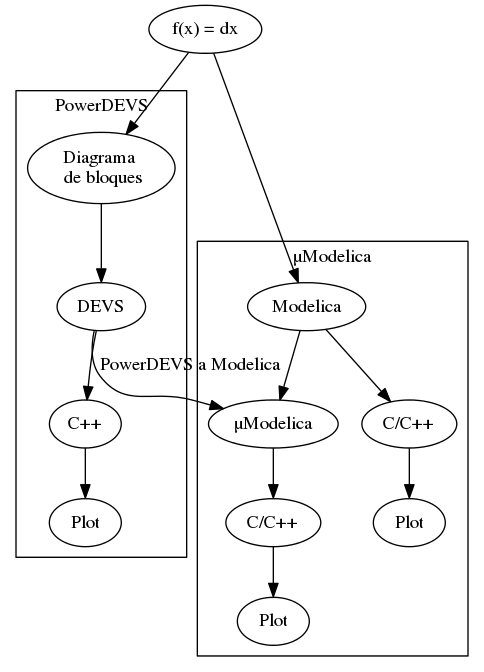
\includegraphics[width=0.75\linewidth]{esquema}
 \caption{Esquema de conversiones}
 \label{fig:esquema}
\end{figure}

En la figura \ref{fig:esquema}, se muestran los dos principales estrategias (PowerDEVS y Modelica) para realizar una simulación. En el caso de PowerDEVS, el primer paso es convertir el sistema en diagramas de bloques, luego en DEVS, en PowerDEVSe el cual puede automáticamente convertirlo en C++ y luego obtener los resultados ejecutando este modelo. Desde la perspectiva de Modelica (o $\mu$modelica, debemos pasar el sistema a modelica (o $\mu$Modelica) y luego el compilador se encargara de generar código (usualmente C o C++) capaz de correr la simulación y obtener resultados.
El actual trabajo esta representado por la flecha que sale de PowerDEVS hacia $\mu$modelica, permitiendo especificar la simulación en diagramas de bloques y ejecutar la simulación en el solver QSS, en el lenguaje $\mu$modelica.

\section{Organización del presente trabajo}

\section{Motivación y Objetivos}
PowerDEVS\cite{BK11} es una herramienta de simulación de sistemas híbridos, basado en el formalismo DEVS\cite{Zeigler:2000:TMS:580780}, con una interfaz gráfica orientada a bloques, donde los bloques pueden ser conectados entre si, modificado sus parámetros, además permite conectarse con el entorno Scilab para poder utilizar expresiones y herramientas de cálculo provistas por este entorno.

La resolución de ecuaciones diferenciales ordinarias, requiere el uso de métodos de integración numérica. Todos los algoritmos tradicionales de integración se basan en la discretización de la variable independiente (que generalmente representa el tiempo).

Las rutinas que implementan estos algoritmos, se denominan solvers y existen gran variedad de implementaciones de los mismos en diferentes lenguajes de programación. Los Métodos de Integración Numérica QSS (Quantized State System), a diferencia de los métodos de integración tradicionales, realizan la discretización sobre las variables de estado. En consecuencia, convierten los sistemas continuos en sistemas de eventos discretos, y tienen grandes ventajas para simular sistemas con discontinuidades.

Si bien PowerDEVS, implementa la totalidad de los algoritmos de QSS, resultan ineficientes, dado que malgastan gran parte de la carga computacional en la transmisión de eventos entre submodelos.

Para solventar este hecho se desarrollo una familia de QSS stand-solver, el cual requiere un modelo descripto en lenguaje C el cual contiene las ecuaciones diferenciales, las funciones de cruce de cero así como la información estructural requerida por los algoritmos QSS. Estos solvers obtienen una mejora de rendimiento de hasta un orden de magnitud comparado con otras implementaciones DEVS.

Sobre este se desarrollo una herramienta la cual genera a partir de un modelo $\mu$-Modedelica \cite{Ber12} (un subconjunto del lenguaje Modelica) el modelo requerido para el QSS solver.

Con el objetivo de utilizar los mejoras de velocidad y mantener un entorno amigable con el usuario, se creo una herramienta capas de convertir un modelo PowerDEVS en un modelo $\mu$modelica.


\section{Trabajo relacionado}
En \cite{Ber12} se describe una extensión del Compilador OpenModelica el cual traslada modelos regulares Modelica a $\mu$modelica. 
ModelicaDEVS \cite{Beltrame06quantisedstate} es una librería Dymola que permite describir simulaciones DEVS en el Modelica, más específicamente en el entorno Dymola.
M/CD++ \cite{conf/mascots/DAbreuW05} es una herramienta para convertir simulaciones en un subconjunto de Modelica, a simulaciones DEVS.
DESlib \cite{Sanz09paralleldevs} es una librería para la descripción de modelos Parallel DEVS en Modelica.


\section{Alcance}
DEVS\cite{Zeigler:2000:TMS:580780}, Discrete Event System Specification (Especificación de Sistemas de Eventos Discretos), es un formalismo modular y jerárquico para modelar y analizar sistemas que pueden ser de eventos de tiempo discreto mediante tablas de transición, y con estados continuos que pueden ser descriptos por ecuaciones diferenciales.
En el formalismo clásico DEVS, los modelos atómicos capturan el comportamiento del sistema, mientras los modelos Acoplados describen la estructura del mismo.
En particular los modelos atómicos en PowerDEVS son descriptos en clases C++, mientras que la estructura se encuentra definida en archivos pds y pdm.
Modelica es un lenguaje de modelado, orientado a objetos, declarativo, para el modelado orientado a componentes de sistemas complejos.
Para poder realizar nuestro objetivo es necesario primero contar con un modelo en modelica\cite{Fritzson02modelica--} para cada atómico PowerDEVS\cite{BK11} que deseemos convertir. 

De esto se desprenden las siguientes limitaciones importantes:
\begin{itemize}
	\item La semántica de los modelos convertidos depende de los modelos equivalentes a los DEVS atómicos 
	\item Solamente podemos convertir modelos cuyos componentes atómicos hayan sido convertidos a $\mu$modelica.
\end{itemize}


